\documentclass[11pt,letter]{article}
\usepackage[top=1.00in, bottom=1.0in, left=1.1in, right=1.1in]{geometry}
\renewcommand{\baselinestretch}{1.5}
\usepackage{graphicx}
\usepackage{natbib}
\usepackage{amsmath}
\usepackage{hyperref}

\def\labelitemi{--}
\begin{document}

\title{`A Fine Balance': Exploring the Interplay of Reproductive Strategies and Growth Dynamics in Trees}
\author{Xiaomao Wang} 
\date{\today}
\maketitle

\setlength{\parindent}{0pt}
\setlength{\parskip}{3pt}

\section{Introduction} 
The fundamental processes in a plant's life cycle—growth, reproduction, defense, and storage, all compete for the same resources. Plants must apply trade-offs to maximize their fitness when the resources are limited. One of the most significant of these trade-offs is the growth-reproduction trade-off, which is influenced by both environmental conditions and the plant's life history strategy. In resource-rich environments, plants are able to allocate resources both to rapid growth and reproduction, while in resource-poor environments, plants often face a decision: they can either allocate resources to growth, ensuring their long-term survival, or they can invest in reproduction, which may come at the expense of growth. This trade-off leads to high variability in reproduction across years, which is manifested as mast seeding, an important reproductive strategy for many plant species. \citep{pearse2016mechanisms}.\par
Mast seeding is the phenomenon of synchronized and variable seed production within plant populations, it is closely related to ecosystem-level functions influencing processes such as seed dispersal, predation and plant recruitment, since seeds can be food resources for many mammals or host for some pathogens  \citep{janzen1971seed, kelly1994evolutionary, davies2024seed}, and also determine the regeneration within a population. It is widely observed in wind-pollinated species, but also occurs in Poaceae as well as Diperocarpaceae \citep{kelly2002mast}. Even though there are several hypotheses explaining the potential mechanism of mast seeding (e.g., predator satiation, resource matching, etc.)  \citep{koenig2021brief}, the exact factors triggering this phenomenon in different species and ecosystems are not fully understood, but appear related to specific climatic conditions that allow trees to build up enough resources to mast  \citep{pearse2016mechanisms}. \par
Masting is distinct from annual fluctuations in seed production in several key ways. It is characterized by four primary features: interannual variation, synchrony, temporal autocorrelation, and frequency \citep{hacket2021climate}. Interannual variation refers to fluctuations in seed production from one year to the next. These fluctuations are not entirely random or caused by immediate environmental conditions but are part of a population-level strategy, with synchrony occurring across large spatial areas, which can extend hundreds of kilometers\citep{kelly1994evolutionary}. Temporal autocorrelation describes the pattern in which a mast year is typically followed by several years of low or no seed production, which distinguishes masting from annual fluctuations. Finally, frequency refers to how often mast years occur, with some species exhibiting a more fixed interval (e.g., every 2-3 years) and others a more irregular pattern (e.g., 2-5 years). Annual fluctuations in seed production, by contrast, are more closely tied to short-term environmental factors and do not exhibit this kind of regularity. \par
A paragraph on how to measure masting\par
Masting plays an important ecological role by influencing seed dynamics and broader ecosystem processes. According to the predator satiation hypothesis, mast years overwhelm seed predators by producing abundant seeds, ensuring that some seeds will survive and germinate. In this way, plants can regulate predator populations and enhance seedling establishment. Mast seeding also contributes to the creation of a seed bank, providing a reserve of seeds for future generations. This strategy not only improves seedling survival in the short term but also promotes long-term regeneration, helping to maintain a plant population over time.
However, with the ongoing climate change, causing the change of growing season and precipitation patterns, plant resources availability is likely to be altered. These changes may influence the balance of the growth-reproduction trade-off and consequently, later masting behavior. Thus, understanding how these dynamics function, and how climate plays the role, is critical for predicting future forest composition and regeneration. Currently, there is no comprehensive model to predict how climate change will affect masting considering the relationship between growth and reproduction across different species and ecosystems, due to the complex and variable nature of mast seeding.\par
The aim of this thesis is to investigate how masting, as a reproductive strategy, is related to the growth dynamics of three species and their role in forest ecoystems, particularly in the context of climate change. Using Mount Rainier as a case study, this research will address three key questions: (1) Which reproductive traits are associated with masting? This help us potentially understand what might trigger the behavior of masting in different environments. (2) Is there a trade-off between mast seeding events and tree growth? (3) How might changing climate conditions affect seed dynamics at Mount Rainier? By answering these questions, this study will contribute to out understanding of how masting shapes the growth and regeneration dynamics of coniferous forests in  Mount Rainier with better models.\par


\section{Explore which reproductive traits are relevant to masting}
Masting is widely observed across different lineages in different biomes, and there are many hypotheses trying to explain in what circumstances masting might had evolutionary benefits compared to those reproduce every year \citep{koenig2021brief, waller1979models}.\par
Different hypotheses try to explain masting from different perspectives. The most commonly accepted hypothesis is the predator satiation hypothesis, which suggests that masting species overwhelm seed predators with a large seed crop, then starve the seed predators during years with a low seed crop \citep{janzen1971seed}. By manipulating the seed predator population, these plants increase the likelihood that their seeds will survive to germinate. Another widely accepted hypothesis is the resource matching hypothesis, which suggests that a fixed fraction of resources is allocated to reproduction every year \citep{kelly1994evolutionary}. The amount of resources available for reproductive output depends on the total resources available to the plants. Another well-known hypothesis is the pollination coupling hypothesis, which claims that environmental conditions and resource availability together determine the flowering effort of plants \citep{crone2014resource}. Highly synchronized flowering improves pollination success and results in more seeds. Closely related to all these hypotheses is the environmental cues hypothesis, which suggests that certain environmental events trigger masting \citep{pearse2016mechanisms}. These hypotheses are not mutually exclusive and may hold true for different species in different environments.\par
Based on these hypotheses, we can link specific traits to the phenomenon of masting. Since masting is a reproductive event, I will focus on reproductive traits the most. Seed reproduction occurs through at least three critical stages: pollination, seed maturation and seed dispersal \citep{satake2021studying}. Each stage presents unique opportunities that can influence the overall success of mast seeding. During the pollination stage, we can link traits to the pollination coupling hypothesis. The critical process during this stage involves flowering traits related to pollination, such as the type of reproduction, whether the plant is monoecious or dioecious, since for dioecious plants, they need individuals of separate genders to accomplish reproduction, so the pollination success might not be as high as monoecious plants when the population density is low \citep{bawa1980evolution}. Thus, I would predict that masting species are more likely to be monoecious. Another important trait is duration of flowering, since a longer flowering period might increase pollination success \citep{knight2005pollen}. It is also generally assumed that masting species tend to be wind-pollinated, so pollination is not restricted by the number of pollinators when large numbers of flowers bloom simultaneously \citep{bogdziewicz2017masting, bogdziewicz2020flowering}. After pollination, fertilized seeds enter the maturation stage, which is more related to the resource matching hypothesis. Traits such as leaf longevity and determinacy, which influence the timing of seed development and a plant's ability to invest in reproduction, are important at this stage. Determinacy defines whether the leaf material is prebuilt or not {lechowicz1984temperate}, it might influence how much resources plants can allocate to reproduction.  Longer leaf longevity facilitate more carbon fixation, which might enhance the resources available for reproduction \citep{adler2014functional}. I predict that determinate species which has their leaf material prebuilt and with longer leaf longevity is more likely to mast. When seeds mature and are ready for dispersal, the role of seed predators becomes crucial. According to the predator satiation hypothesis, in masting years, plants overwhelm seed predators by producing large numbers of seeds. On the other hand, masting species may also rely on seed dispersers to carry seeds away from the parent tree, increasing the chances of seedling survival \citep{janzen1971seed, silvertown1980evolutionary}. In this context, seed traits such as seed size, nutrient content, dispersal mode, seed dormancy and seed longevity all can play important roles. Larger seeds with higher nutrient content might be more attractive to seed predators. Seed dormancy and seed longevity help ensure that seeds do not germinate immediately after dispersal, allowing them to wait for better conditions to establish in a more favorable environment since mast events only occur once every few years.\par

\begin{figure}[htb]
	\centering
	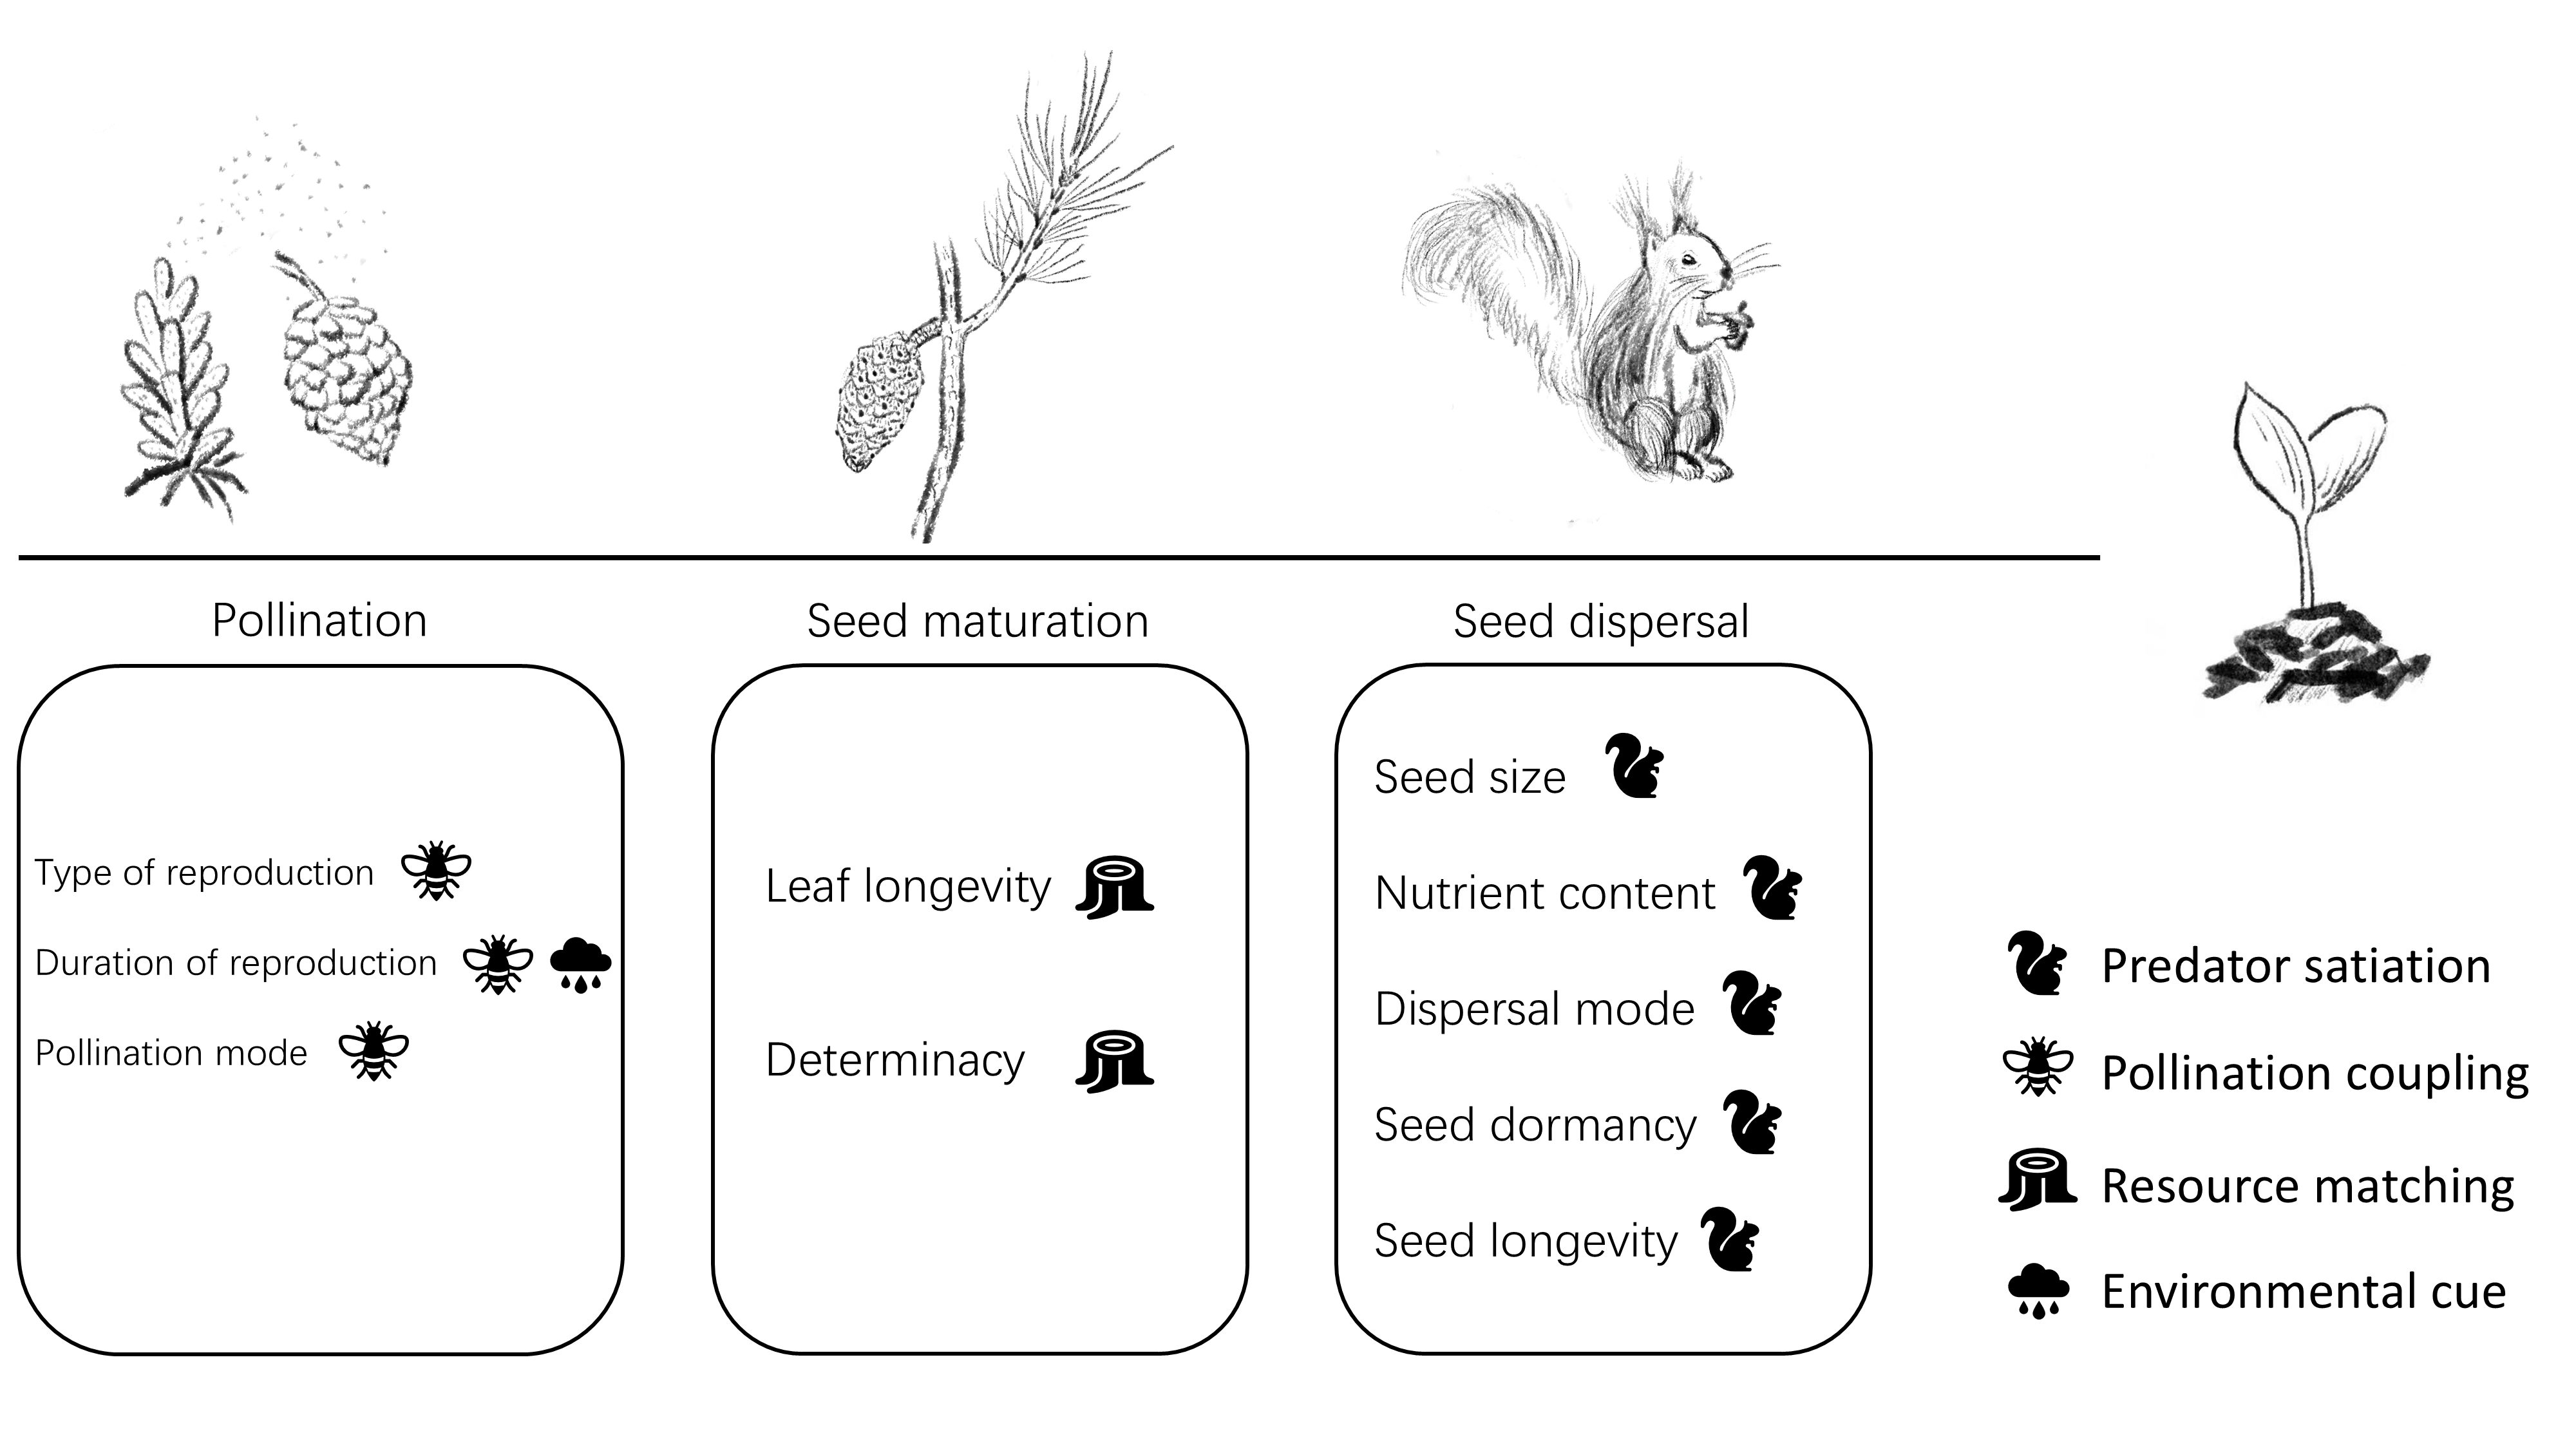
\includegraphics[width=1\linewidth]{conceptualChap1.png}
	\caption{Conceptual framework linking reproductive traits to the phenomenon of masting across critical stages of seed reproduction.}
	\label{fig:conceptual1}
\end{figure}
There are several preliminary studies explored the relationship between some traits with interannual variability in seed production. Their results provided some evidences for different hypotheses \citep{journe2023evolution, fernandez2019nutrient, pearse2020biogeography}, but did not explain in different environments, which reproductive traits might be critical determine whether the decision of a species to mast would be successful or not. In this meta-analysis, I will include reproductive traits associated with different hypotheses to investigate how these traits are related to a species' tendency to mast in different forest types and biomes.\par

\subsection{Research Question and Objectives}
Which seed traits are related to masting, and what might cause masting in different species?
	\begin{itemize}
	\item \textbf{Investigate Trait Associations:} Analyze the relationships between specific reproductive traits and masting event and frequency to determine which traits maybe advantages in masting.
	\item \textbf{Compare across Different Environments:} Compare the most critical traits across different forest types and biomes to determine if they vary.
	\end{itemize}
\subsection{Methods}
This chapter aims to explore the relationship between reproductive traits and the tendency of a species to mast in various environments through a meta-analysis.\par
\textbf{Data collection}\\
Data for this meta-analysis will be primarily sourced from following resources:
	\begin{itemize}
	\item \textbf{Silvics of North America:} This resource will provide a comprehensive database of tree species and their reproductive characteristics in North America, this is going to be our main dataset. It includes flowering traits, seed dispersal traits, mast cycles and forest types we are interested in.
	\item \textbf{MASTREE+:} This is a specialized database focusing on tree species and their mast seeding behavior, which will be a supplement source for identifying species tendencies for mast seeding and interannual variability.
	\item \textbf{Kew Seed Dataset, Worldwide Seed Mass Dataset, USDA Seed Manual:} These sources will offer supplementary information on seed mass and other reproductive traits.
	\end{itemize}
\textbf{Statistical Analysis and Model Development}\\
The main analysis will involve logistic regression to determine the likelihood of mast seeding based on the selected reproductive traits and environmental variables. The response variables, whether a species mast or not and CV will be analyzed separately to evaluate the occurrence and variability of mast seeding behavior.
\subsection{Significance} 
Studying the reproductive traits related to masting can provide valuable insights into reproductive strategies and the broader ecological impacts on forest ecosystems. First, it can help explain the potential mechanisms that drive this complex reproductive strategy, shedding light on why certain species mast while others do not in different environments. By examining traits such as seed size, nutrient content, dormancy, and longevity, researchers can gain insights into how these characteristics influence the success of seed production and dispersal during mast years, and how this is related to the seed predator's population dynamics.\par
Additionally, understanding these relationships can help us to predict how environmental factors, such as climate change, may impact masting behavior in the future. For example, knowing which seed traits are most relevant to masting behavior in specific ecological contexts can help us anticipate how shifts in temperature, precipitation, and other environmental cues might change masting patterns. By answering the question of what causes masting through looking at seed traits, we can better understand the dynamics of forest ecosystems.\par

\section{Understanding the relationship between masting and growth}
Plants have limited resources and must allocate them efficiently to support survival and reproduction. The basic processes in the life cycle of plants include vegetative growth, sexual or asexual reproduction, defense and storage \citep{bazzaz1997plant}. How plants allocate their resources depends on both environmental conditions and their life history strategy. Given these constraints, plants cannot maximize all aspects of their life processes simultaneously, and thus trade-offs become crucial for their fitness.\par
One fundamental trade-off in plant ecology is the growth-reproduction trade-off, which suggests that increased investment in one process often comes at the expense of the other\citep{stearns1998evolution}. For trees, the decision to allocate resources to a large seed crop during a masting year may significantly affect their overall growth dynamics \citep{hacket2016tree}, particularly for species that require multiple years to complete their reproductive cycles. With anthropogenic climate change, tree growth in generally expected to increase, as warmer temperatures enhance growth rates and provide trees with more time to growth each year with extended growing season \citep{keenan2014net, finzi2020carbon}. Most climate models predict a positive relationship between temperature and growth \citep{ito2020global, friedlingstein2022global}. However, recent studies have questioned whether the extending of growing seasons due to warming has actually led to increased tree growth \citep{dow2022warm, green2022limits}.  Studies have suggested that biotic factors, such as intrinsic species differences and how plants allocate the additional carbon gained during warmer seasons, also play a significant role \citep{hacket2016consistent}. In terms of masting, this relationship might become even more complicated, but it is important for us to understand future behavior of different tree species.\par
\begin{figure}[htb]
	\centering
	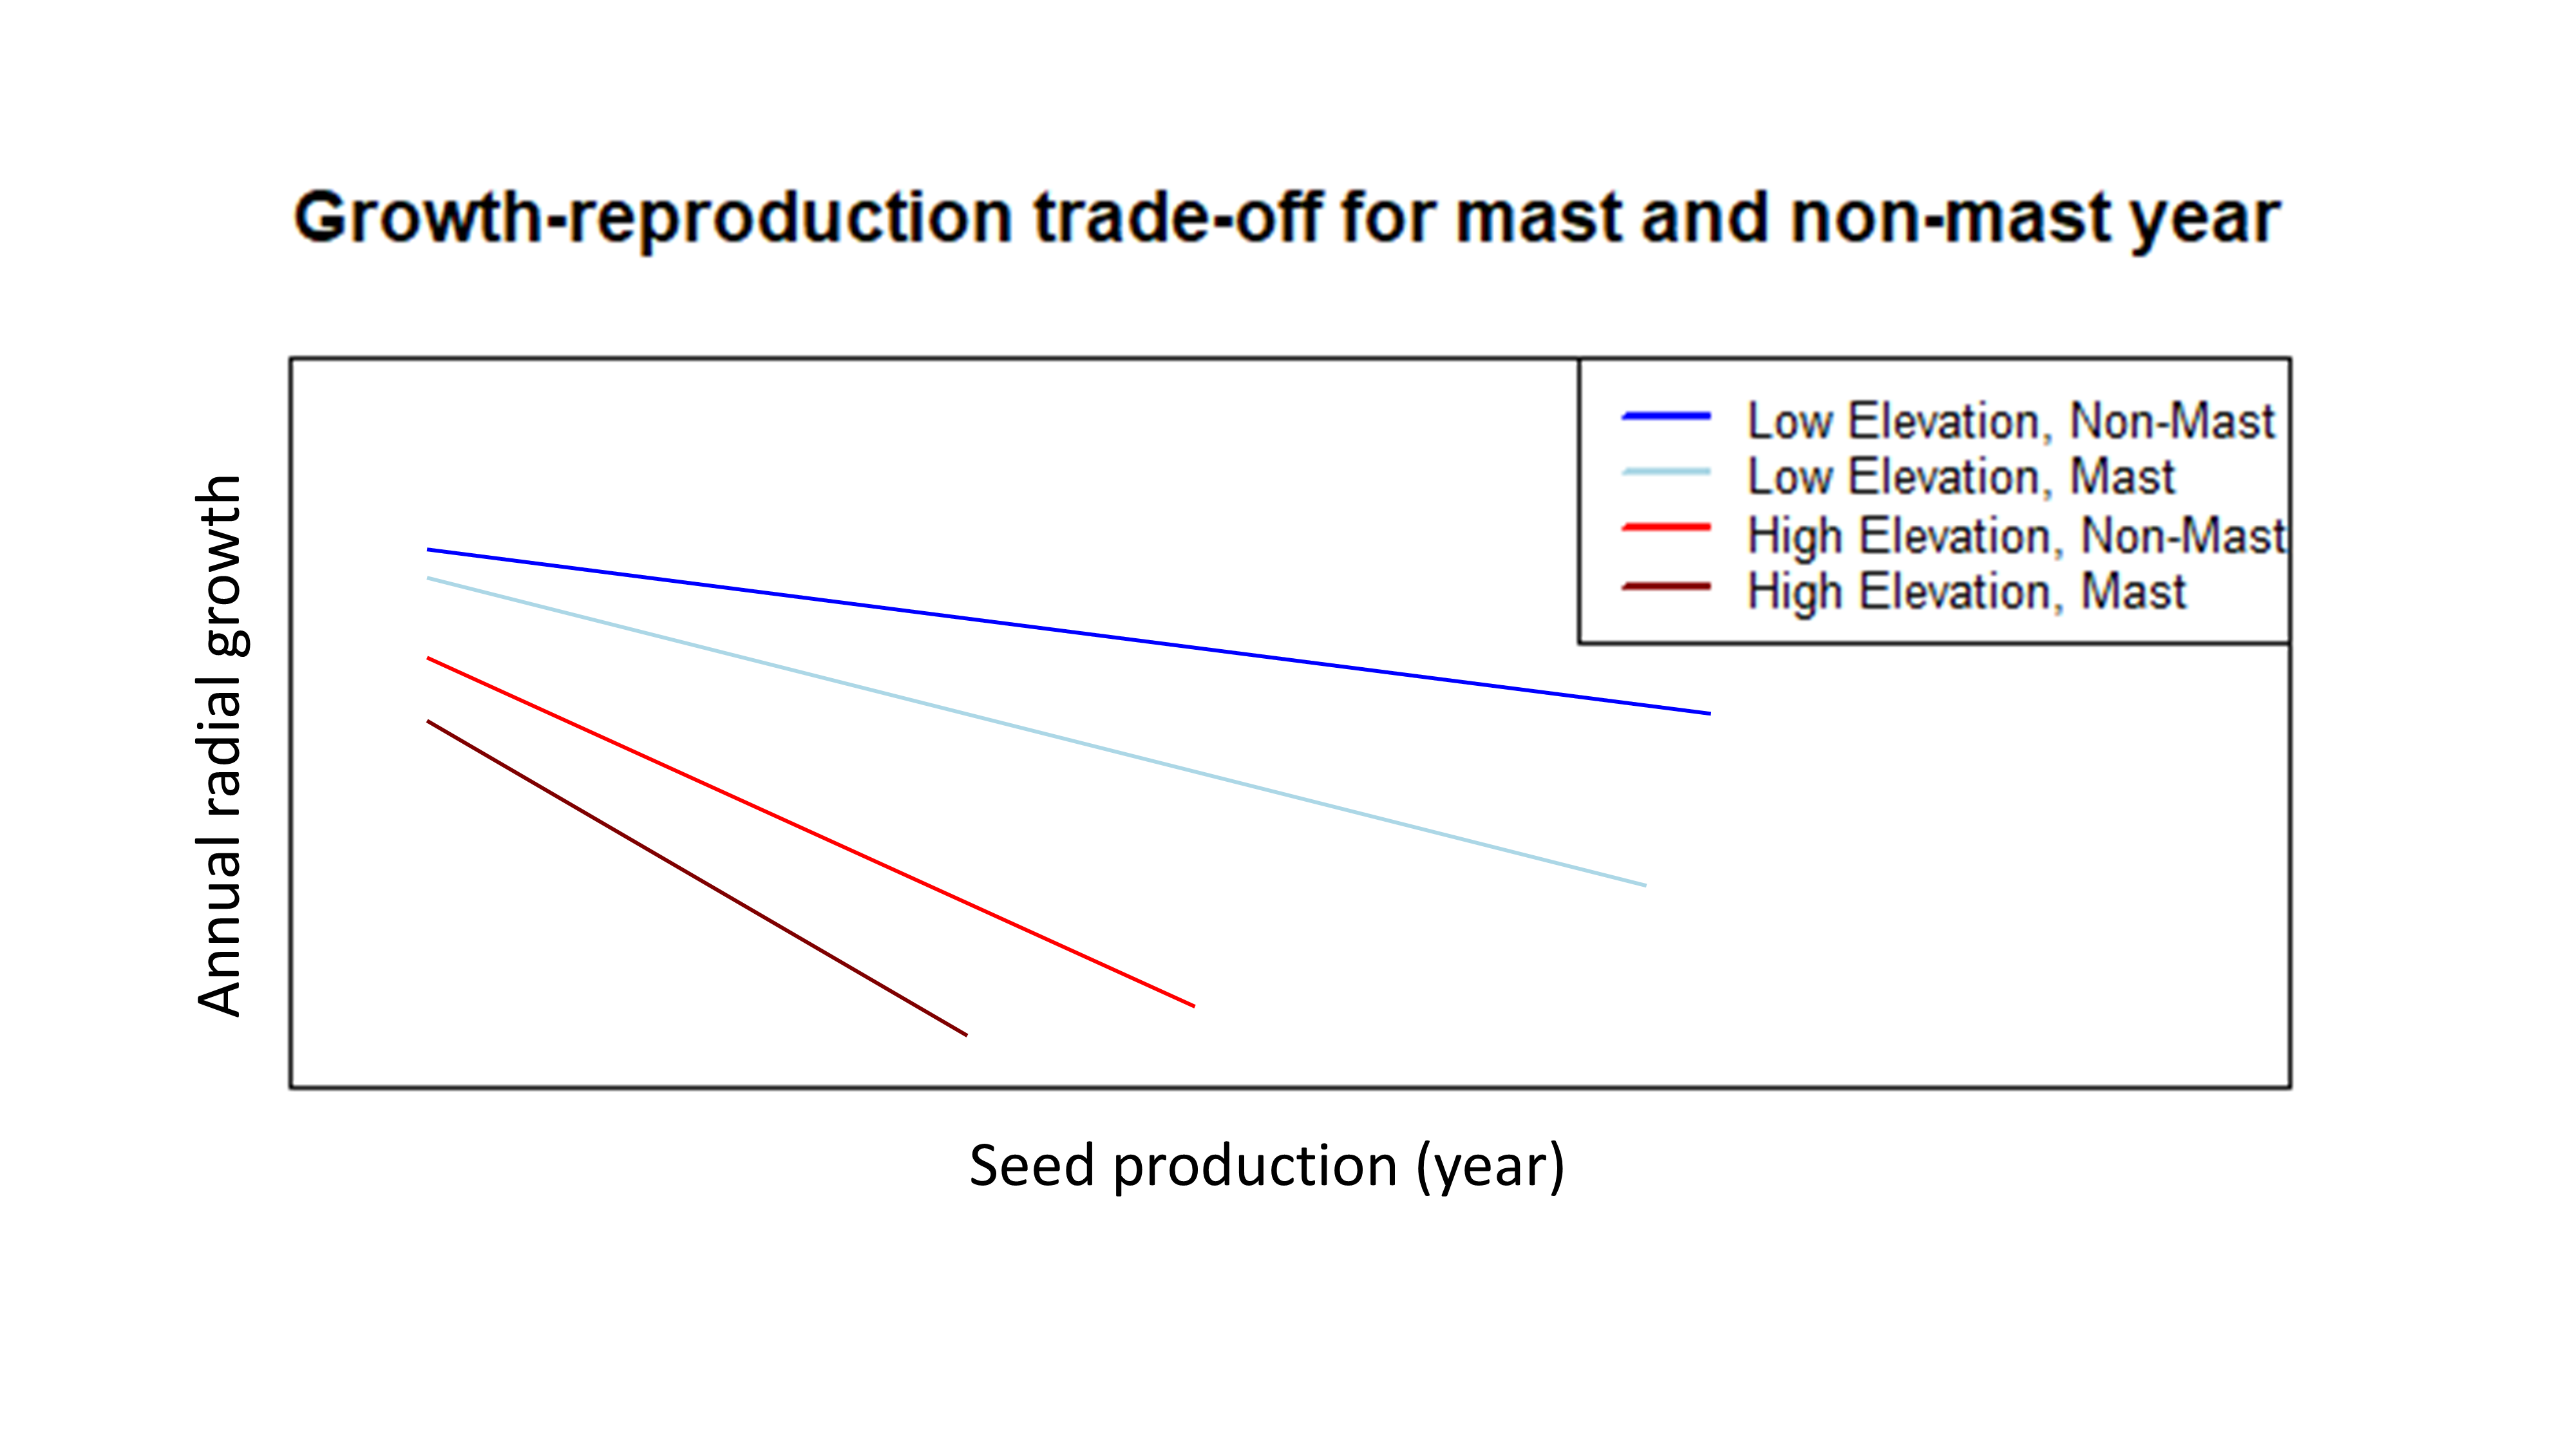
\includegraphics[width=1\linewidth]{conceptualFigureChap2.png}
	\caption{A conceptual figure showing the expected trend of growth-reproduction trade-off in masting year and non-masting year at different elevations. I would expect that the trade-off is more pronounced in masting years compared to non-masting years in general and individuals at higher elevation would experience a higher trade-off}
	\label{fig:conceptual2}
\end{figure}
Previous studies have made complex conclusions regarding the trade-offs between growth and reproduction during masting years. While many studies have focused on how climate affects both growth and reproduction, and compared how these processes respond to different climate factors \citep{koenig2020can, bajocco2021characterizing, redmond2019resource, sanchez2011trade}, few have directly investigated the growth-reproduction trade-off in the context of masting. Research focusing on oak species has shown mixed results, with little evidence of a strong, consistent response in radial growth relative to seed production \citep{koenig2020can, patterson2023acorn}. However, these studies have not entirely ruled out the possibility that radial growth could be used to understand masting patterns. Mast seeding and growth responses can vary significantly among tree species, especially across different elevations, where resource availability and environmental stresses differ. Species with different allocation strategies will also respond uniquely in environments with varying resource levels. For instance, trees at higher elevations may exhibit a more pronounced trade-off between growth and reproduction, driven by limited resources. Species with a more conservative strategy might also have a more pronounced trade-off as they allocate resources to ensure their growth in resource-limited conditions.\par
By combining Mount Rainier's unique elevational gradient with long-term tree growth data from tree rings, this chapter will explore the relationship between mast seeding and growth in six common coniferous tree species at Mount Rainier, emphasizing the trade-offs that influence reproductive strategies and how these strategies may vary across ecological conditions.\par

\subsection{Research Question and Objectives}
Is there a more pronounced trade-off between mast seeding events and growth?
	\begin{itemize}
	\item \textbf{Assess Growth Patterns:} Analyze the historical annual growth of selected tree species in relation to their masting events to determine if there exist a trade-off.
	\item \textbf{Compare Species Responses:} Evaluate the differences in masting and growth responses among various tree species across different elevations with various resources allocation strategies.
	\end{itemize}

\subsection{Methods}
\begin{table}[htb]
	\centering
	\small
	\caption{Targeted species}
\begin{tabular}{|p{5cm}|p{5cm}|p{5cm}|}
\hline
 Tree species & Common name & Life history strategies\\ \hline %emw13Nov: italicize latin binomials 
\textit{Abies amabilis} & Pacific silver fir & Conservative \\ \hline
\textit{Pseudotsuga menziesii} & Douglas fir & Acquisitive    \\\hline
\textit{Tsuga heterophylla} & Western hemlock & Conservative    \\\hline
\textit{Tsuga mertensiana} & Mountain hemlock & Conservative    \\\hline
\textit{Thuja plicata} & Western redcedar & Conservative    \\\hline
\textit{Callitropsis nootkatensis} & Yellow cedar & Conservative    \\\hline
\end{tabular}
\end{table}
This chapter aims to examine the growth-reproduction trade-off in relation to mast seeding for six common conifer species at Mount Rainier across different elevations. To explore this relationship, I will incorporate long-term seed trap data with historical growth data derived from tree core samples, and use statistical approaches to analyze their relationship.\par
\textbf{Study site and sample collection}\\
\begin{figure}[htb]
	\centering
	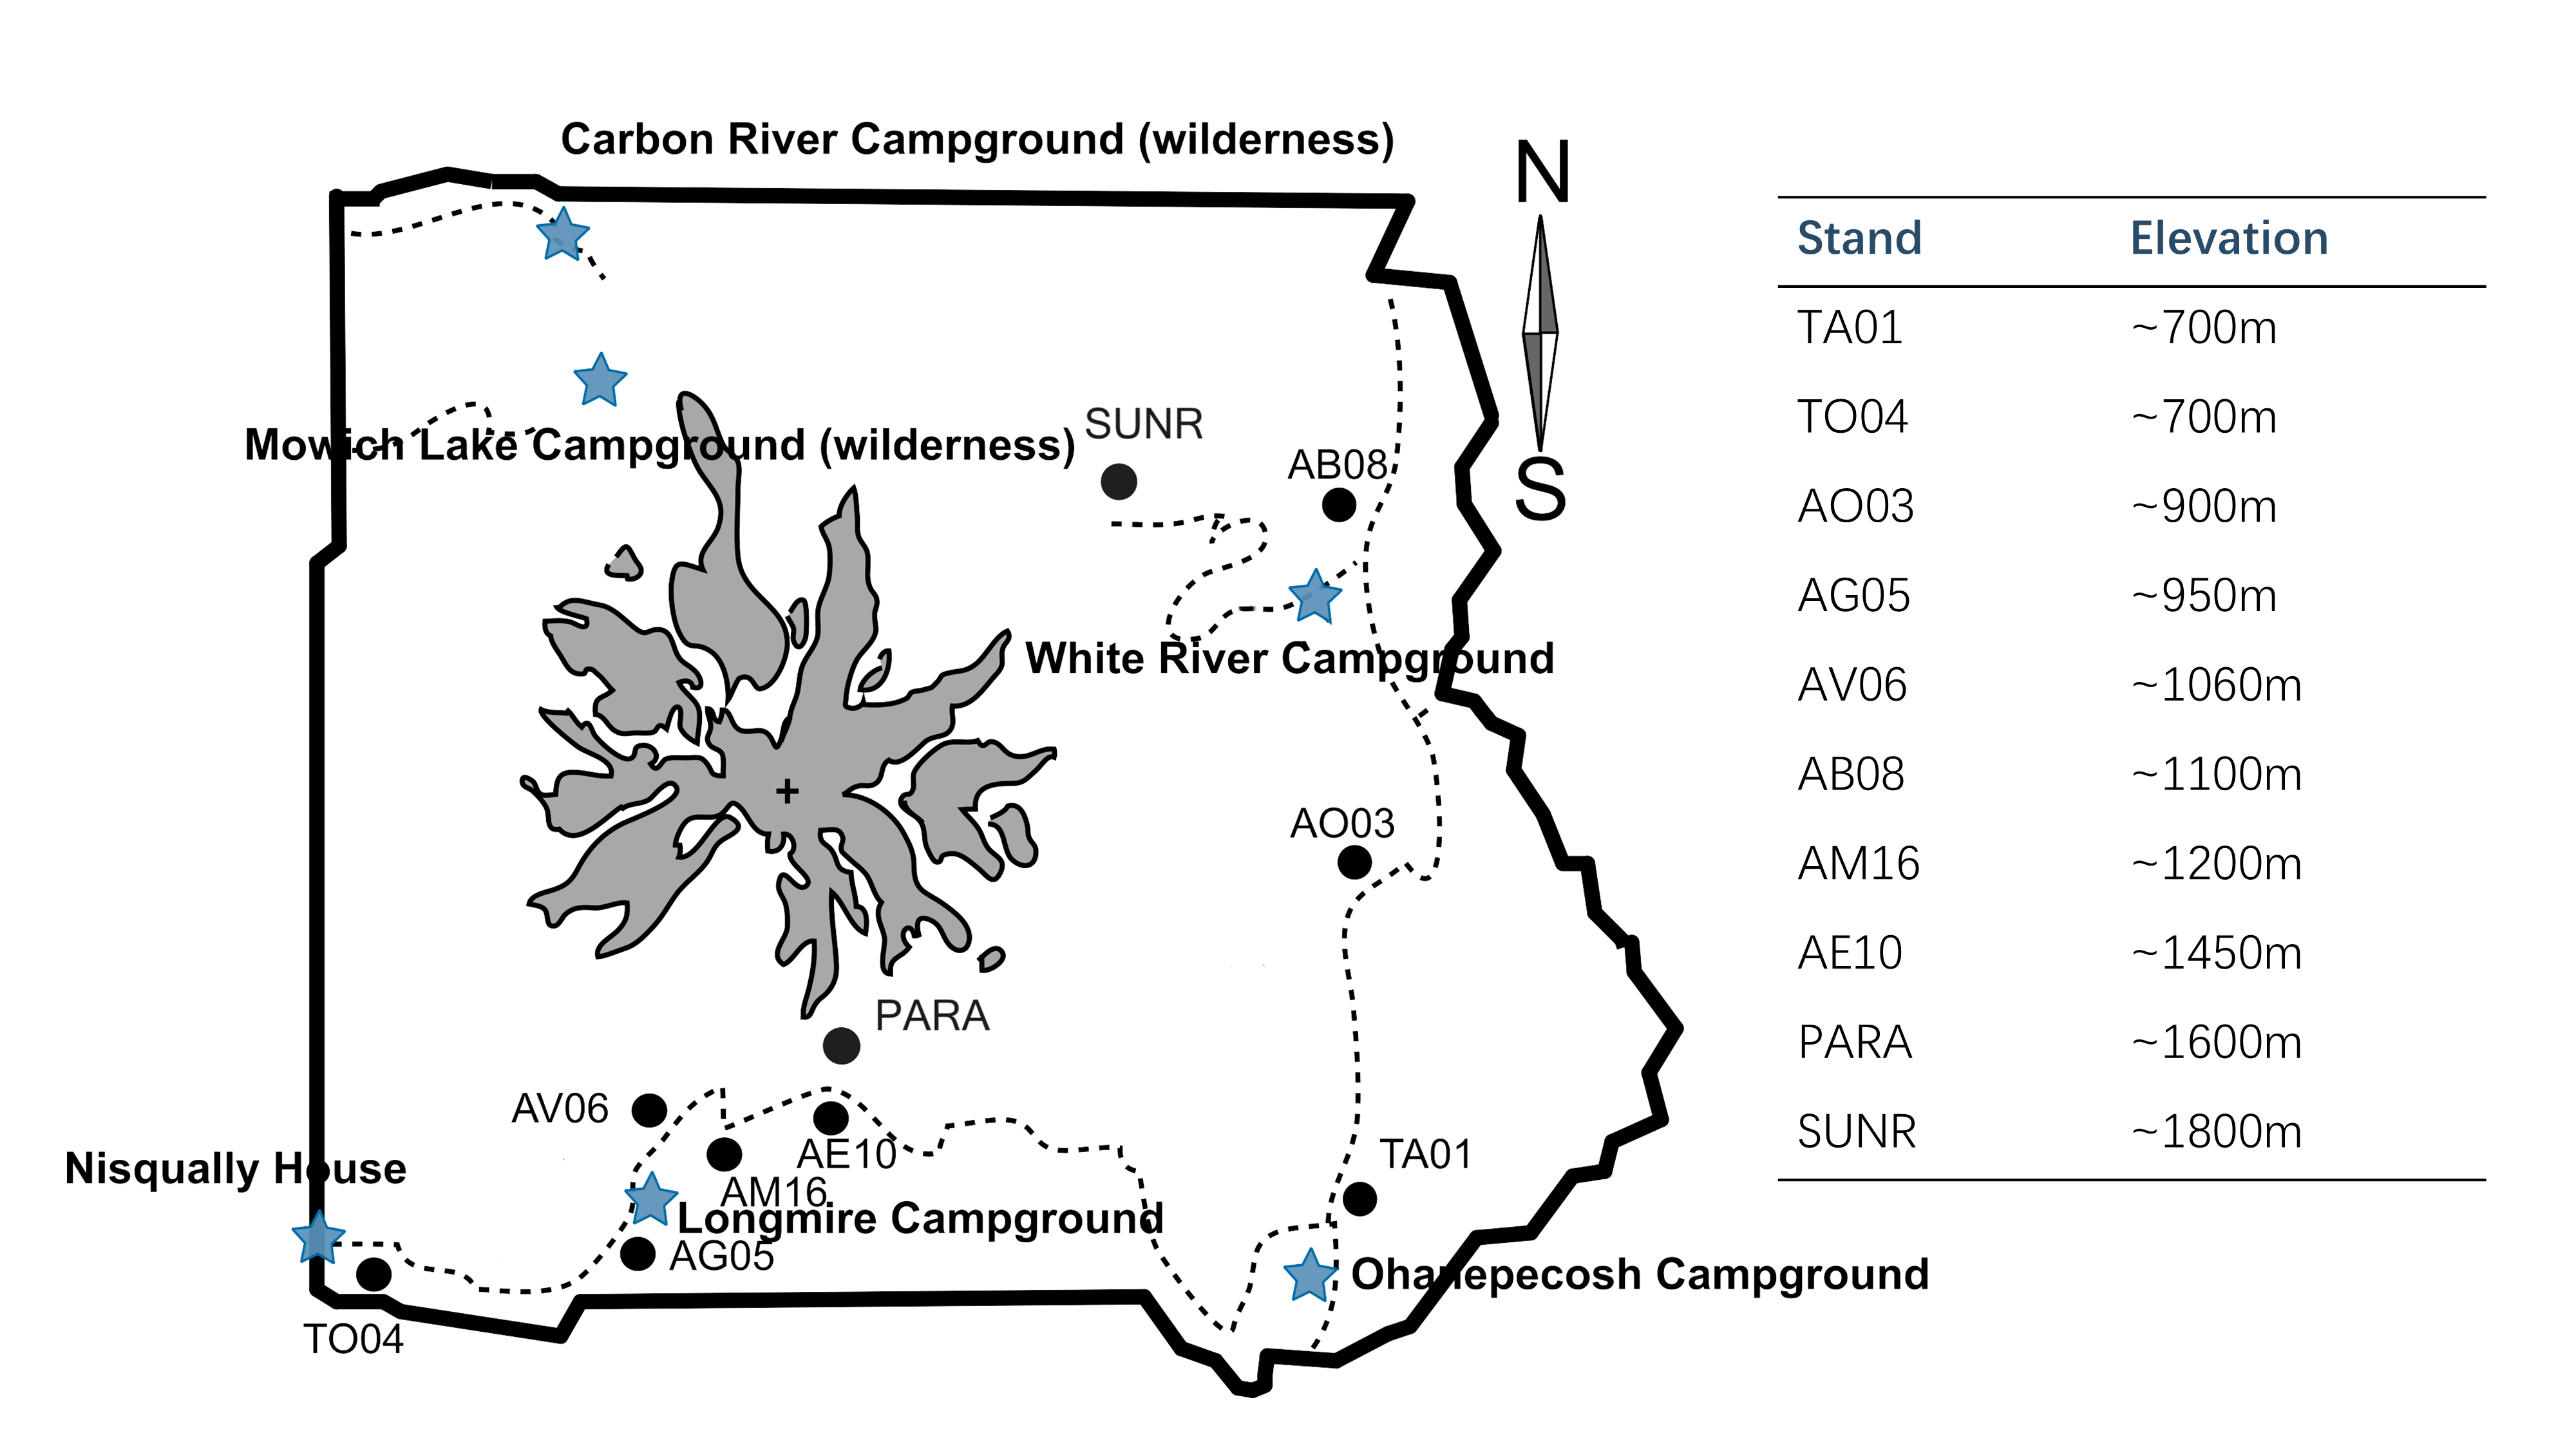
\includegraphics[width=1\linewidth]{rainierMap.png}
	\caption{A map of Mount Rainier with all the sampling sites for this study}
	\label{fig:sites}
\end{figure}\\
This study is conducted in Mount Rainier National Park, Washington, USA. We will focus on six common conifer species that exhibit varying masting behaviors and occur across different elevations in the park. The data I am going to use in this chapter include two components:
\begin{itemize}
	\item \textbf{Long-term seed data:} Our collaborator Janneke Hille Ris Lambers, has been collecting stand-level seed production data using seed traps since 2008. These data provide a valuable record of masting events across different stands and elevations at Mount Rainier.
	\item \textbf{Tree growth data:}  To assess the historical growth of individual trees, I will collect cores from targeted species listed above in each stand with long-term seed data. Within each stand, there are at least 2 targeted species, and each species appears in at least 4 stands. I plan to collect tree cores from 25 individuals per species per stand, covering a size gradient. To make sure the trees we core were mature enough to reproduce at least 10 years ago, I will only collect from trees with DBH greater than 25cm. Additionally, I will prioritize individuals that are close to seed traps to better correlate with seed data. I will core trees at breast height using increment borers, taking two tree cores from the opposite sides of the tree while avoiding slopes. To account for at least 15 years of growth and for cross-dating purposes, I will collect long cores of 25 cm from larger trees with a DBH above 50 cm, while for smaller trees, I will core to the center if possible.
	\end{itemize}
\begin{figure}[htb]
	\centering
	\includegraphics[width=1\linewidth]{seed.png}
	\caption{Seed data across all 10 stands collected by seed traps from 2009-2017 at Mount Rainier. Both the total seeds (filled seeds + empty seeds) and only filled seeds are shown in this figure. Short blue arrows indicate potential masting years.}
	\label{fig:sites}
\end{figure}	
\textbf{Tree core processing}\\
I will prepare the cores for analysis by sanding them with fine grits sandpaper (up to 2000 grit depending on the visibility of rings) to ensure a smooth, clear surface. For cores with rings that are difficult to distinguish, I will use a microtome to further enhance the visibility of the rings, creating a clear surface for better quality.\par
After preparation, I will scanned the cores using a high-resolution camera to capture detailed images of the growth rings, then I will analyzed the images with CooRecorder, a software used to measure tree ring width. I will also double check the cross-dating results with COFECHA.
\textbf{Statistical analysis}\\
I will use multivariate models to analyze the relationship between growth and reproduction.

\subsection{Significance}
Understanding the relationship between masting and growth is important for predicting how tree species will respond to changing environmental factors, particularly in the context of extending growing season, how trees might allocate additional carbon. By examining how these processes interact, we can gain insights into the adaptive strategies of different species and their potential resilience or vulnerability to future climate changes. This knowledge allows us to make more informed predictions about future forest dynamics, including shifts in species composition, regeneration, and ecosystem health. As climate conditions continue to fluctuate, understanding the  masting behavior and growth responses will be essential for effective forest management and conservation efforts, helping us to anticipate changes and make strategies that will support the sustainability and resilience of forest ecosystems.\par

\section{Investigate how changing climate affect masting dynamics}
Plants need to assimilate enough resources to produce seeds, a process that requires a combination of environmental conditions such as light, water, nutrients and suitable temperature. These factors can directly influence mast seeding by affecting seed development process or affect it indirectly by regulating flowering or growth. Flowering, for instance, is regulated by day length, and light plays a key role by influencing the production of hormones which control both flowering and growth \citep{lau2010plant}. Light is also a critical element for photosynthesis, which supports healthy plant growth. Water is another essential element for both flowering and fruiting. It helps maintain optimal turgor pressure, which is necessary for proper flower development, while also facilitating nutrient transport and supporting cell expansion \citep{taiz2002plant}. When water availability is limited, plants may conserve energy, leading to fewer or smaller flowers, reduced pollination success, or even shedding flowers before maturation. After fertilization, water continues to play a crucial role in the expansion and maturation of seeds. Beside its direct effects on reproduction, water stress also inhibits growth, limiting the resources available for reproduction \citep{hsiao1973plant, anjum2011morphological}. Nutrients, both macronutrients and micronutrients, are essential for both energy transfer and storage, playing a significant role in the formation of flowers and seed development. Nutrient availability influences the timing of lowering and seed formation, with well-nourished plants more likely to flower at the appropriate time and set seeds successfully. One of the most widely studied climatic factors linked to masting events is temperature \citep{bajocco2021characterizing, moreira2015effects, schauber2002masting, bogdziewicz2024evolutionary}, especially spring temperature, which is crucial period for the meiosis of pollen and ovules.\par
To understand how climate change may impact masting events, it is important to explore the relationship between environmental factors and mast seeding behavior first. Mast seeding is characterized by four main features: interannual variation, synchrony, temporal autocorrelation, and frequency. These characteristics are all likely to be affected by climate change in different ways \citep{hacket2021climate}. Once we have a sense of how different environmental factors are manipulating different aspects of masting, we can make better prediction of how future changing climate might shape the seed dynamics in this region. One significant change expected with climate change is the extension of the growing season, which may allow trees to allocate more carbon to growth and reproduction \citep{keenan2014net}. This shift could have profound implications for the frequency and intensity of masting events. Additionally, warmer temperatures could increase the frequency of droughts, which would limit water supply. On the other hand, in areas with year-round snow cover, temperature changes may alter water dynamics, affecting the timing and availability of water. Another critical factor in the flowering and fruiting process is environmental vetoes, which refer to conditions where weather events or environmental factors prevent certain processes in a plant, even when the plant has sufficient resources \citep{bogdziewicz2022will} . Environmental vetoes can take two forms: (1) a lack of weather cues, such as when specific weather conditions required to trigger flowering or fruit maturation are not met, preventing reproduction despite adequate resources; and (2) extreme weather events, such as frost, drought, or heavy rainfall, which can directly damage plant tissues, including shoots, flowers and fruits, thereby preventing successful reproduction. With climate change, it is likely that environmental vetoes will become more frequent, which is generally considered detrimental to plants. However, studies have shown that environmental vetoes preventing seed production in certain years can actually facilitate masting, allowing for higher regeneration success \citep{bogdziewicz2018correlated, bogdziewicz2019environmental}. Therefore, understanding how environmental vetoes influence seed production in different species and regions is critical for predicting future forest dynamics.\par
Elevation is closely linked to a variety of climatic factors, particularly temperature and water availability, and has long been used as a proxy for climate change in ecological studies. It provides a natural system to study the long-term, large-scale effects of climate change on communities and ecosystems which cannot be accomplished by experiments \citep{sundqvist2013community}. By using elevation as a proxy for climate change, we can better understand how plant populations at different elevations respond to environmental factors and refine predictive models that incorporate shifting climatic variables at finer spatial resolutions. This approach also helps us understand ecosystem and vegetation shifts within a region.\par
Mount Rainier provides an ideal location for studying how climate change may impact forest dynamics, as it features a distinct elevation la gradient and diverse snowmelt patterns. The rain shadow effect on different sides of the mountain also creates varying water availability. The climate in this region has already undergone significant changes in recent decades, and by combining historical seed data with climate data, we can explore the relationship between climatic variables and various aspects of mast seeding. This will allow us to make more accurate predictive models.
This chapter aims to identify common patterns in masting influenced by environmental factors. By investigating the large variance in interannual masting patterns, and exploring the relationship between spatial as well as temporal changes in masting across elevational gradients, we can better understand how climate change will impact seed dynamics in this area.\par
\subsection{Research Question and Objectives}
How does changing climate affect seed dynamics at Mount Rainier?
\begin{itemize}
\item\textbf{Identify Environmental Influences:} Investigate how key environmental factors (e.g., temperature, precipitation) are related to masting events at Mount Rainier.
\item\textbf{Climate change proxy:} Use the elevational gradient at Mount Rainier as a proxy for changing climate conditions to compare how masting behavior varies across different elevations.
\item\textbf{Develop Predictive Models:} Develop predictive models of masting behavior across elevations to forecast future seed dynamics under changing climate conditions.
\end{itemize}
\subsection{Methods}
This chapter aims to investigate how climate change influences seed dynamics at Mount Rainier, focusing on the relationship between mast seeding patterns adapted to local climatic conditions across different elevations for the same species. By using long-term seed trap data and corresponding climate data, I will assess how seed production synchrony and variability change along the elevation, which is used as a proxy for climate change for same species we used in last chapter.
\textbf{Data collection}\\
\begin{itemize}
\item\textbf{Long-term seed data:} The same long-term seed trap data from last chapter.
\item\textbf{Local climate data:}
\end{itemize}
\textbf{Statistical Analysis and Model Development}\\
\begin{itemize}
\item\textbf{Time series model, mixed-effect models:}
\item\textbf{Predictive modeling:} I will develop predictive models to forecast future trends in masting behaviours at Mount Rainier under projected climate scenarios. These models will use climate projections for this retion to predict how seed dynamics might shift in response to future climate change.
\end{itemize}
\subsection{Significance}
Changes in masting behavior can have cascading effects on forest dynamics, including seed predator interactions and the regeneration success of tree species. Since masting events can provide a large food source drives population dynamics of lots of mammals in the forest, changes of masting patterns will alter these ecological relationships, and further the overall structure of ecosystems. Fore example, if climate change causes masting events to be less synchronized across species or elevations, it will affect seed availability for animals that rely on them as food source, potentially impacting their survival and reproduction.
Masting will also affect the regeneration of tree species itself. Many tree species rely on mast seeding years to establish successful new seedlings in the face of competition and predation. If climate change affects the frequency or intensity of mast seeding events, the successful regeneration of some tree species might be adversely affected. Thus, understanding how these characteristics of masting might be influenced by climate change is essential for predicting the resilience of forest ecosystems.


\bibliographystyle{besjournals}
\bibliography{Proposal} 
\end{document}